% Created by tikzDevice version 0.12.6 on 2025-04-07 16:48:33
% !TEX encoding = UTF-8 Unicode
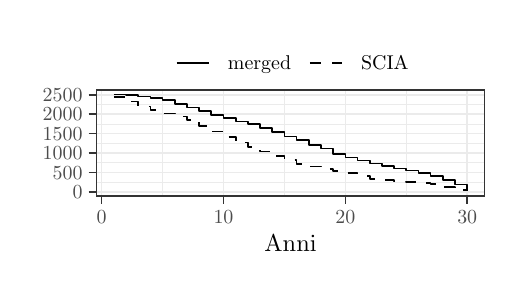
\begin{tikzpicture}[x=1pt,y=1pt]
\definecolor{fillColor}{RGB}{255,255,255}
\path[use as bounding box,fill=fillColor] (0,0) rectangle (170.72, 88.20);
\begin{scope}
\path[clip] (  0.00,  0.00) rectangle (170.72, 88.20);
\definecolor{drawColor}{RGB}{255,255,255}

\path[draw=drawColor,line width= 0.6pt,line join=round,line cap=round,fill=fillColor] (  0.00,  0.00) rectangle (170.72, 88.20);
\end{scope}
\begin{scope}
\path[clip] ( 24.75, 27.29) rectangle (165.22, 65.79);
\definecolor{fillColor}{RGB}{255,255,255}

\path[fill=fillColor] ( 24.75, 27.29) rectangle (165.22, 65.79);
\definecolor{drawColor}{gray}{0.92}

\path[draw=drawColor,line width= 0.3pt,line join=round] ( 24.75, 32.30) --
	(165.22, 32.30);

\path[draw=drawColor,line width= 0.3pt,line join=round] ( 24.75, 39.34) --
	(165.22, 39.34);

\path[draw=drawColor,line width= 0.3pt,line join=round] ( 24.75, 46.38) --
	(165.22, 46.38);

\path[draw=drawColor,line width= 0.3pt,line join=round] ( 24.75, 53.42) --
	(165.22, 53.42);

\path[draw=drawColor,line width= 0.3pt,line join=round] ( 24.75, 60.46) --
	(165.22, 60.46);

\path[draw=drawColor,line width= 0.3pt,line join=round] ( 48.75, 27.29) --
	( 48.75, 65.79);

\path[draw=drawColor,line width= 0.3pt,line join=round] ( 92.78, 27.29) --
	( 92.78, 65.79);

\path[draw=drawColor,line width= 0.3pt,line join=round] (136.81, 27.29) --
	(136.81, 65.79);

\path[draw=drawColor,line width= 0.6pt,line join=round] ( 24.75, 28.79) --
	(165.22, 28.79);

\path[draw=drawColor,line width= 0.6pt,line join=round] ( 24.75, 35.82) --
	(165.22, 35.82);

\path[draw=drawColor,line width= 0.6pt,line join=round] ( 24.75, 42.86) --
	(165.22, 42.86);

\path[draw=drawColor,line width= 0.6pt,line join=round] ( 24.75, 49.90) --
	(165.22, 49.90);

\path[draw=drawColor,line width= 0.6pt,line join=round] ( 24.75, 56.94) --
	(165.22, 56.94);

\path[draw=drawColor,line width= 0.6pt,line join=round] ( 24.75, 63.98) --
	(165.22, 63.98);

\path[draw=drawColor,line width= 0.6pt,line join=round] ( 26.73, 27.29) --
	( 26.73, 65.79);

\path[draw=drawColor,line width= 0.6pt,line join=round] ( 70.76, 27.29) --
	( 70.76, 65.79);

\path[draw=drawColor,line width= 0.6pt,line join=round] (114.80, 27.29) --
	(114.80, 65.79);

\path[draw=drawColor,line width= 0.6pt,line join=round] (158.83, 27.29) --
	(158.83, 65.79);
\definecolor{drawColor}{RGB}{0,0,0}

\path[draw=drawColor,line width= 0.6pt,line join=round] ( 31.13, 64.04) --
	( 35.54, 64.04) --
	( 35.54, 63.94) --
	( 39.94, 63.94) --
	( 39.94, 63.39) --
	( 44.34, 63.39) --
	( 44.34, 62.74) --
	( 48.75, 62.74) --
	( 48.75, 62.01) --
	( 53.15, 62.01) --
	( 53.15, 60.71) --
	( 57.55, 60.71) --
	( 57.55, 59.33) --
	( 61.96, 59.33) --
	( 61.96, 58.04) --
	( 66.36, 58.04) --
	( 66.36, 56.63) --
	( 70.76, 56.63) --
	( 70.76, 55.48) --
	( 75.17, 55.48) --
	( 75.17, 54.28) --
	( 79.57, 54.28) --
	( 79.57, 53.28) --
	( 83.97, 53.28) --
	( 83.97, 51.94) --
	( 88.38, 51.94) --
	( 88.38, 50.45) --
	( 92.78, 50.45) --
	( 92.78, 48.89) --
	( 97.18, 48.89) --
	( 97.18, 47.52) --
	(101.59, 47.52) --
	(101.59, 45.83) --
	(105.99, 45.83) --
	(105.99, 44.48) --
	(110.39, 44.48) --
	(110.39, 42.64) --
	(114.80, 42.64) --
	(114.80, 41.24) --
	(119.20, 41.24) --
	(119.20, 40.22) --
	(123.60, 40.22) --
	(123.60, 39.09) --
	(128.01, 39.09) --
	(128.01, 38.33) --
	(132.41, 38.33) --
	(132.41, 37.26) --
	(136.81, 37.26) --
	(136.81, 36.57) --
	(141.22, 36.57) --
	(141.22, 35.60) --
	(145.62, 35.60) --
	(145.62, 34.54) --
	(150.03, 34.54) --
	(150.03, 33.22) --
	(154.43, 33.22) --
	(154.43, 31.47) --
	(158.83, 31.47) --
	(158.83, 29.60);

\path[draw=drawColor,line width= 0.6pt,dash pattern=on 4pt off 4pt ,line join=round] ( 31.13, 63.12) --
	( 35.54, 63.12) --
	( 35.54, 61.49) --
	( 39.94, 61.49) --
	( 39.94, 59.76) --
	( 44.34, 59.76) --
	( 44.34, 58.46) --
	( 48.75, 58.46) --
	( 48.75, 57.24) --
	( 53.15, 57.24) --
	( 53.15, 56.15) --
	( 57.55, 56.15) --
	( 57.55, 54.87) --
	( 61.96, 54.87) --
	( 61.96, 52.73) --
	( 66.36, 52.73) --
	( 66.36, 50.63) --
	( 70.76, 50.63) --
	( 70.76, 48.59) --
	( 75.17, 48.59) --
	( 75.17, 46.66) --
	( 79.57, 46.66) --
	( 79.57, 45.16) --
	( 83.97, 45.16) --
	( 83.97, 43.43) --
	( 88.38, 43.43) --
	( 88.38, 41.89) --
	( 92.78, 41.89) --
	( 92.78, 40.48) --
	( 97.18, 40.48) --
	( 97.18, 39.02) --
	(101.59, 39.02) --
	(101.59, 38.09) --
	(105.99, 38.09) --
	(105.99, 37.19) --
	(110.39, 37.19) --
	(110.39, 36.29) --
	(114.80, 36.29) --
	(114.80, 35.60) --
	(119.20, 35.60) --
	(119.20, 34.63) --
	(123.60, 34.63) --
	(123.60, 33.47) --
	(128.01, 33.47) --
	(128.01, 33.14) --
	(132.41, 33.14) --
	(132.41, 32.67) --
	(136.81, 32.67) --
	(136.81, 32.32) --
	(141.22, 32.32) --
	(141.22, 32.02) --
	(145.62, 32.02) --
	(145.62, 31.60) --
	(150.03, 31.60) --
	(150.03, 30.59) --
	(154.43, 30.59) --
	(154.43, 29.45) --
	(158.83, 29.45) --
	(158.83, 29.04);
\definecolor{drawColor}{gray}{0.20}

\path[draw=drawColor,line width= 0.6pt,line join=round,line cap=round] ( 24.75, 27.29) rectangle (165.22, 65.79);
\end{scope}
\begin{scope}
\path[clip] (  0.00,  0.00) rectangle (170.72, 88.20);
\definecolor{drawColor}{gray}{0.30}

\node[text=drawColor,anchor=base east,inner sep=0pt, outer sep=0pt, scale=  0.72] at ( 19.80, 26.32) {0};

\node[text=drawColor,anchor=base east,inner sep=0pt, outer sep=0pt, scale=  0.72] at ( 19.80, 33.36) {500};

\node[text=drawColor,anchor=base east,inner sep=0pt, outer sep=0pt, scale=  0.72] at ( 19.80, 40.40) {1000};

\node[text=drawColor,anchor=base east,inner sep=0pt, outer sep=0pt, scale=  0.72] at ( 19.80, 47.44) {1500};

\node[text=drawColor,anchor=base east,inner sep=0pt, outer sep=0pt, scale=  0.72] at ( 19.80, 54.48) {2000};

\node[text=drawColor,anchor=base east,inner sep=0pt, outer sep=0pt, scale=  0.72] at ( 19.80, 61.52) {2500};
\end{scope}
\begin{scope}
\path[clip] (  0.00,  0.00) rectangle (170.72, 88.20);
\definecolor{drawColor}{gray}{0.20}

\path[draw=drawColor,line width= 0.6pt,line join=round] ( 22.00, 28.79) --
	( 24.75, 28.79);

\path[draw=drawColor,line width= 0.6pt,line join=round] ( 22.00, 35.82) --
	( 24.75, 35.82);

\path[draw=drawColor,line width= 0.6pt,line join=round] ( 22.00, 42.86) --
	( 24.75, 42.86);

\path[draw=drawColor,line width= 0.6pt,line join=round] ( 22.00, 49.90) --
	( 24.75, 49.90);

\path[draw=drawColor,line width= 0.6pt,line join=round] ( 22.00, 56.94) --
	( 24.75, 56.94);

\path[draw=drawColor,line width= 0.6pt,line join=round] ( 22.00, 63.98) --
	( 24.75, 63.98);
\end{scope}
\begin{scope}
\path[clip] (  0.00,  0.00) rectangle (170.72, 88.20);
\definecolor{drawColor}{gray}{0.20}

\path[draw=drawColor,line width= 0.6pt,line join=round] ( 26.73, 24.54) --
	( 26.73, 27.29);

\path[draw=drawColor,line width= 0.6pt,line join=round] ( 70.76, 24.54) --
	( 70.76, 27.29);

\path[draw=drawColor,line width= 0.6pt,line join=round] (114.80, 24.54) --
	(114.80, 27.29);

\path[draw=drawColor,line width= 0.6pt,line join=round] (158.83, 24.54) --
	(158.83, 27.29);
\end{scope}
\begin{scope}
\path[clip] (  0.00,  0.00) rectangle (170.72, 88.20);
\definecolor{drawColor}{gray}{0.30}

\node[text=drawColor,anchor=base,inner sep=0pt, outer sep=0pt, scale=  0.72] at ( 26.73, 17.41) {0};

\node[text=drawColor,anchor=base,inner sep=0pt, outer sep=0pt, scale=  0.72] at ( 70.76, 17.41) {10};

\node[text=drawColor,anchor=base,inner sep=0pt, outer sep=0pt, scale=  0.72] at (114.80, 17.41) {20};

\node[text=drawColor,anchor=base,inner sep=0pt, outer sep=0pt, scale=  0.72] at (158.83, 17.41) {30};
\end{scope}
\begin{scope}
\path[clip] (  0.00,  0.00) rectangle (170.72, 88.20);
\definecolor{drawColor}{RGB}{0,0,0}

\node[text=drawColor,anchor=base,inner sep=0pt, outer sep=0pt, scale=  0.88] at ( 94.98,  7.21) {Anni};
\end{scope}
\begin{scope}
\path[clip] (  0.00,  0.00) rectangle (170.72, 88.20);
\definecolor{fillColor}{RGB}{255,255,255}

\path[fill=fillColor] ( 52.41, 76.79) rectangle (137.56, 82.70);
\end{scope}
\begin{scope}
\path[clip] (  0.00,  0.00) rectangle (170.72, 88.20);
\definecolor{fillColor}{RGB}{255,255,255}

\path[fill=fillColor] ( 52.41, 68.25) rectangle ( 66.86, 82.70);
\end{scope}
\begin{scope}
\path[clip] (  0.00,  0.00) rectangle (170.72, 88.20);
\definecolor{drawColor}{RGB}{0,0,0}

\path[draw=drawColor,line width= 0.6pt,line join=round] ( 53.85, 75.48) -- ( 65.42, 75.48);
\end{scope}
\begin{scope}
\path[clip] (  0.00,  0.00) rectangle (170.72, 88.20);
\definecolor{fillColor}{RGB}{255,255,255}

\path[fill=fillColor] (100.52, 68.25) rectangle (114.98, 82.70);
\end{scope}
\begin{scope}
\path[clip] (  0.00,  0.00) rectangle (170.72, 88.20);
\definecolor{drawColor}{RGB}{0,0,0}

\path[draw=drawColor,line width= 0.6pt,dash pattern=on 4pt off 4pt ,line join=round] (101.97, 75.48) -- (113.53, 75.48);
\end{scope}
\begin{scope}
\path[clip] (  0.00,  0.00) rectangle (170.72, 88.20);
\definecolor{drawColor}{RGB}{0,0,0}

\node[text=drawColor,anchor=base west,inner sep=0pt, outer sep=0pt, scale=  0.72] at ( 72.36, 73.01) {merged};
\end{scope}
\begin{scope}
\path[clip] (  0.00,  0.00) rectangle (170.72, 88.20);
\definecolor{drawColor}{RGB}{0,0,0}

\node[text=drawColor,anchor=base west,inner sep=0pt, outer sep=0pt, scale=  0.72] at (120.48, 73.01) {SCIA};
\end{scope}
\end{tikzpicture}
